\section{Experiment One Results} \label{results-1-quan}
In this section, we first describe the demographic distribution of the participants. Then, we present the descriptive statistics of the data in our first experiment. Lastly, we discuss results from our Bayesian analysis approach.

\subsection{Participant Demographics}
% -- raw data
%     describe the dataset, total # of participants in each group before and after dataset cleaning, demographics of each group;
    
We collected 223 complete responses in the first experiment.  We removed four poor-quality responses where participants responded the qualitative question facetiously or they misunderstood the prompt. Among the 219 remaining responses, 56 completed the Likert path. Since the remaining participants each completed two of the three QV surveys with 36 credits (QV36), 108 credits (QV108) and 324 credits (QV324) in random, we collected 107 responses for QV36, 108 for QV108 and 111 for QV324. 
\tc{Since we have more variations of experiment conditions for the QV group (choosing two of the three versions with randomized order), and that Bayesian analysis is less sensitive to the number of participants, we collected much more QV participant from the experiment without collecting more participants for the Likert survey group.}
%(To-do: maybe add a hierarchical graph the represents how responses from different paths are aggregated)

We recruited the participants to match the demographic distribution in the US 2018 census estimates in terms of age and education level, as shown in \Cref{table:demo_exp1}. This reduced bias from the sample and allowed more balanced voices from different subgroups of the population, which is generally hard to achieve in MTurk studies without specific control \cite{difallah2018demographics}. Having a representative sample is critical to ensure the generalizability of voting and survey tools. 


\begin{table}
  \centering
  \caption{Experiment one sample demographics statistics align closely with \lwt{2018} US census across all groups and subgroup. Of a total of 219 experimental subjects, 56 subjects took the Likert scale survey, 107 subjects took the QV36 survey, 108 the QV108 survey and 111 subjects took the QV324 survey.} \label{table:demo_exp1}
  \sisetup{
    table-number-alignment = center, 
    table-figures-integer = 2, 
    table-figures-decimal = 2,
    round-mode = figures,
    round-precision = 3,
    detect-weight=true
    % mode=text
  } \begin{tabularx}{0.98\textwidth}
    {@{}>{\raggedleft\arraybackslash}XSSSS>{\bfseries}SS@{}}
    \toprule
    Demographics & {Likert (\si{\percent})} &  {QV36 (\si{\percent})} & {QV108 (\si{\percent})} & {QV324 (\si{\percent})} & {All (\si{\percent})} & {Census (\si{\percent})} \\
    \midrule
    \textsc{\bfseries Education} & &   &  & & &\\
    No High School & 16.07  & 14.02  & 13.89  & 14.41  & 14.61  & 10.22  \\
    High School & 25.00  & 27.10  & 25.93  & 26.13  & 26.03  & 27.73  \\
    College  Associate & 28.57  & 26.17  & 34.26  & 34.23  & 32.88  & 33.09  \\
    Bachelor's Degree and above & 30.36  & 32.71  & 34.26  & 34.23  & 32.88  & 33.09  \\ 
    \textsc{\bfseries Age} & & & & & &\\
    18--24 & 21.43  & 15.89  & 14.81  & 15.32  & 16.89  & 13.65  \\
    25--39 & 26.79  & 29.91  & 30.56  & 29.73  & 29.22  & 30.74  \\
    40--54 & 25.00  & 29.91  & 28.70  & 29.73  & 28.31  & 28.32  \\
    55--69 & 26.79  & 24.30  & 25.93  & 25.23  & 25.57  & 27.29  \\
    \bottomrule\end{tabularx}
\end{table}

Overall, 48.18\% of the participants identified with male, 50.45\% with female, 0.9\% with non-binary, and 1 preferred not to disclose. As for the distribution of races, 77.27\% of the participants were White, 11.82\% were Asian, 9.09\% were Black or African American, 1.36\% were other races and one of them did not disclose the information. These distributions among each group closely resembled one another.

\subsection{Descriptive Statistics}
% donation descriptive statistics: perc of non-zero donation, total donation amount comparison across groups, donation distribution across topics between groups


Since cosine similarity angle, our metric that measured the degree of alignment between survey responses and donation amount, could not take on all-zero vectors, we could only analyze participants who donated a non-zero amount. Therefore, we further filtered the dataset to keep only the responses that had a non-zero total donation amount. Across all the conditions, the average non-zero donation rate was $73.3\%$, consistent with the results provided by \textcite{fehr2007human} in \citeyear{fehr2007human}, which suggested that about $30\%$ of the population would always free-ride in public goods provision regardless of what others do. The number of valid responses after dropping zero-donation participants for Likert, QV36, QV108, and QV324 were $44$, $76$, $76$ and $84$ respectively.
% The donation rate in each condition closely centered around the average donation rate, ranging from $70.37\%$ (in QV108) and $77.19\%$ (in Likert).

Overall, we found that the total amount of donation per participant was large enough to be distributed across charities in a way that could represent the full picture of their true underlying preferences for nine topics in most cases. Among those who donated a non-zero amount, about 60\% of them donated part of the lottery winning amount (\$5 - \$20) but still kept a significant portion for themselves. Another 25\% of the participants contributed a majority of the lottery reward ($\geq \$33$), if not the full amount. The total donation amount distribution across four surveying methods were relatively consistent, except that almost twice the proportion of participants in the Likert condition donated almost the full amount compared to the other QV conditions. For more details, please refer to \Cref{total_donation}.


% Aggregated across all participants,
% the amount of donations for each 
% of the nine charities have a similar trend
% shown in Figure \ref{fig:topic_don_exp1}. 
% Environment-related, health-related, and human-related charities 
% were consistently the more popular 
% compared to the art-related, international-related, and faith-related charities.
% However, there are some differences 
% when observing the population-level preferences 
% towards charities across the four surveying methods. 
% For example, the pets-related charity 
% received far less donation in percentage 
% for the Likert Group compared with the QV groups. 
% This suggests that there was a good amount of variance 
% in people's opinions toward the nine topics, 
% making the surveying task meaningful.

% \begin{figure}[htpb]
%     \centering
%     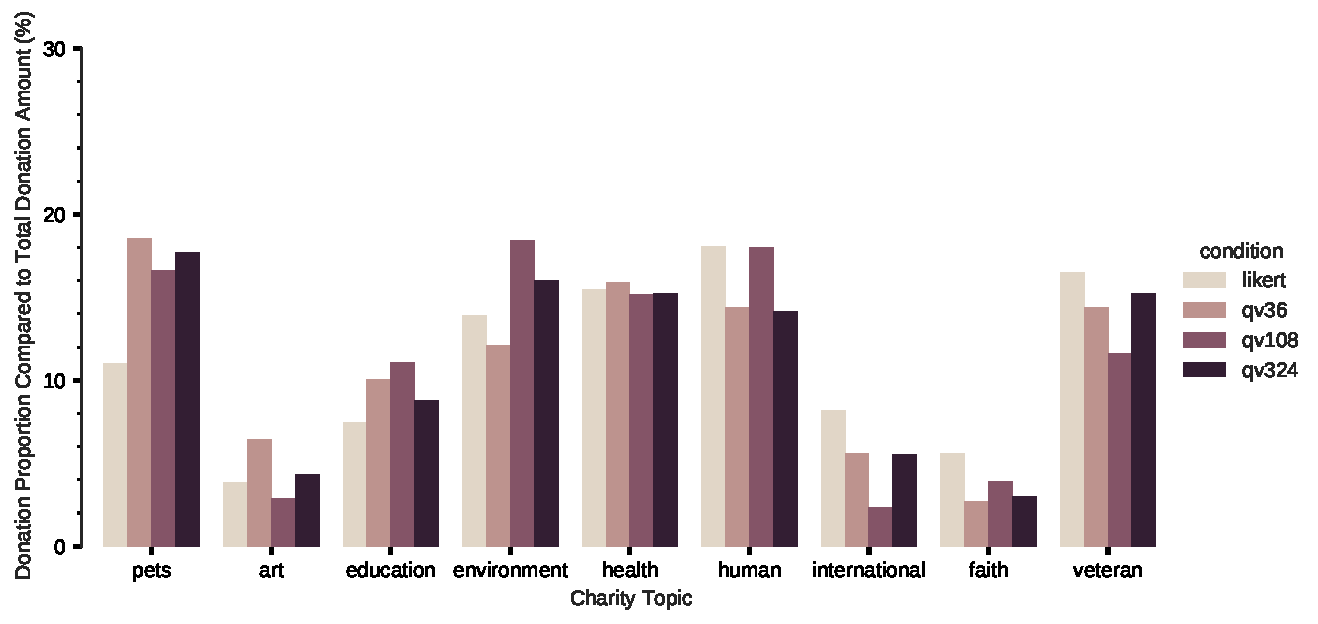
\includegraphics[width=\textwidth, keepaspectratio=true]{content/image/normalized_contributions_per_topic_across_conditions.pdf}
%     \caption{
%       Percentage Contribution Amount per Topic with Respect to the Total Donation Amount across Conditions.
%       We see a general trend of the more and less popular charities while some differences across each
%       surveying method within each group.
%     }
%     \Description[Percentage Contribution Amount per Topic with Respect to the Total Donation Amount across Conditions for experiment 1]{
%       Percentage Contribution Amount per Topic with Respect to the Total Donation Amount across Conditions.
%       We see a general trend of the more and less popular charities while some differences across each
%       surveying method within each group.
%     }
%     \label{fig:topic_don_exp1}
% \end{figure}

\begin{figure}[htpb]
    \centering
    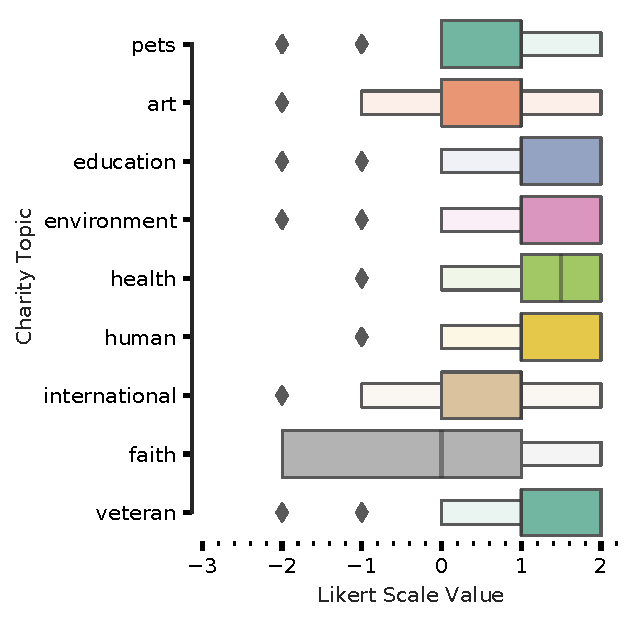
\includegraphics[width=0.4\textwidth, keepaspectratio=true]{content/image/likert_distribution_per_topic.pdf}
    \caption{
      Distribution of Likert scale responses per societal causes in Boxen plot. 
      Each level from -2 to 2 corresponds to 
      ``Very unimportant'', ``Unimportant'', ``Neutral'', ``Important'', and ``Very important''.
      The distributions across all groups vary in their shapes, suggesting that participants showed their relative preferences even in the Likert group.
    }
    \Description[Distribution of Likert Scale Responses per Topic for experiment one in Boxen plot]{Distribution of Likert Scale Responses per Topic for experiment one in Boxen plot}
    \label{fig:likert_exp1}
\end{figure}

%     QV & Likert votes descriptive statistics: votes distribution per topic across groups, budget usage distribution across QV groups

\Cref{fig:likert_exp1} shows the sample distributions of Likert responses across the nine societal causes. Distributions of most topics skewed towards positive opinions, with a median of either "Important" or "Very Important." Despite six out of nine topics had the same median of "Important," the shapes of their distributions were different, suggesting that participants expressed different levels of support based on their relative preferences. 
% The sufficient amount of variations shown across topics indicated that our prompt in the experiment, which we reminded participants that resources are limited and one should express their relative preferences worked as intended. 

Comparing across the three QV surveys, the response distributions were similar but had subtle differences (\Cref{fig:qv3_exp1}). Most distributions of all the topics approximated a Normal distribution, consistent with prior work by \textcite{quarfoot2017quadratic}. The medians of the distributions in QV36 varied less compared to those in QV108 and QV324. As the number of available voice credits increased, we found no decrease in the median of percentage budget usage -- all around 98\% (for details, refer to \Cref{fig:qv_budget_exp1} in the Appendix). This finding suggested that participants made effective use of the extra credits when completing QV with a large budget up to the order of $N^2$ ($N$ is the number of options in a survey) with our QV interface despite more complicated calculations. 
% but the tail of lower percentage usage in QV324 was longer then in the other two cases. 

% mention the implication of longer tail in QV324 in the discussion section: 
% need to be aware of using an overly large budget and resulting in a worse tail

\begin{figure}[htpb]
    \centering
    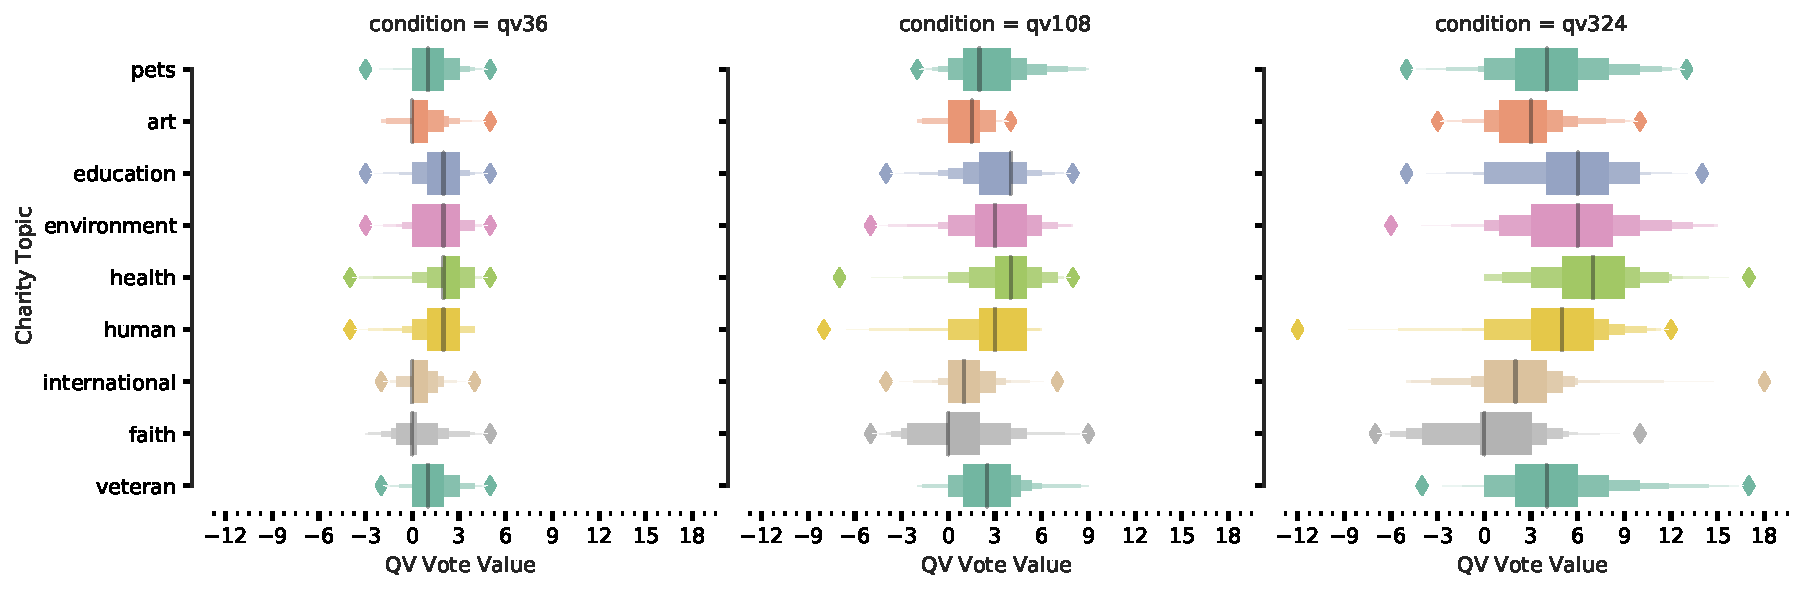
\includegraphics[width=\textwidth, keepaspectratio=true]{content/image/qv_distribution_per_topic.pdf}
    \caption{
      Distribution of QV responses per societal causes in QV36, QV108 and QV324 in Boxen plots. The maximum possible number of votes on a topic was 6 votes in QV36, 10 votes in QV108, and 18 votes in QV324. Most distributions in all three QV set-ups follow a normal distribution. The medians of the distributions in QV36 varied less compared to those in QV108 and QV324. The tails stretch out longer as the number of total credits increases. 
    }
    \Description[Distribution of QV Responses per Topic for experiment one]{Distribution of QV Responses per Topic for experiment one}
    \label{fig:qv3_exp1}
\end{figure}

% Visualize the raw voting and donation data together to show covariation
Since we are interested in the alignment between survey responses and donation behaviors, to get an intuitive view of how they correlate with each other, we visualize the correlation between the normalized survey responses (between -1 and 1) and the proportional donation amount of every participant in \Cref{fig:topic_covariate_exp1}. For all subplots, the points approximately followed a trend line with a positive slope, indicating a potential positive correlation between survey responses and donation behaviors. Within each topic, the slopes of the fitted lines in QV were more positive than that of Likert in most cases, suggesting a stronger correlation between QV survey responses and donation behaviors. To examine rigorously about how aligned the survey responses were with the donation behaviors in different conditions, we present the results from our Bayesian analysis.

\begin{figure}[htpb]
    \centering
    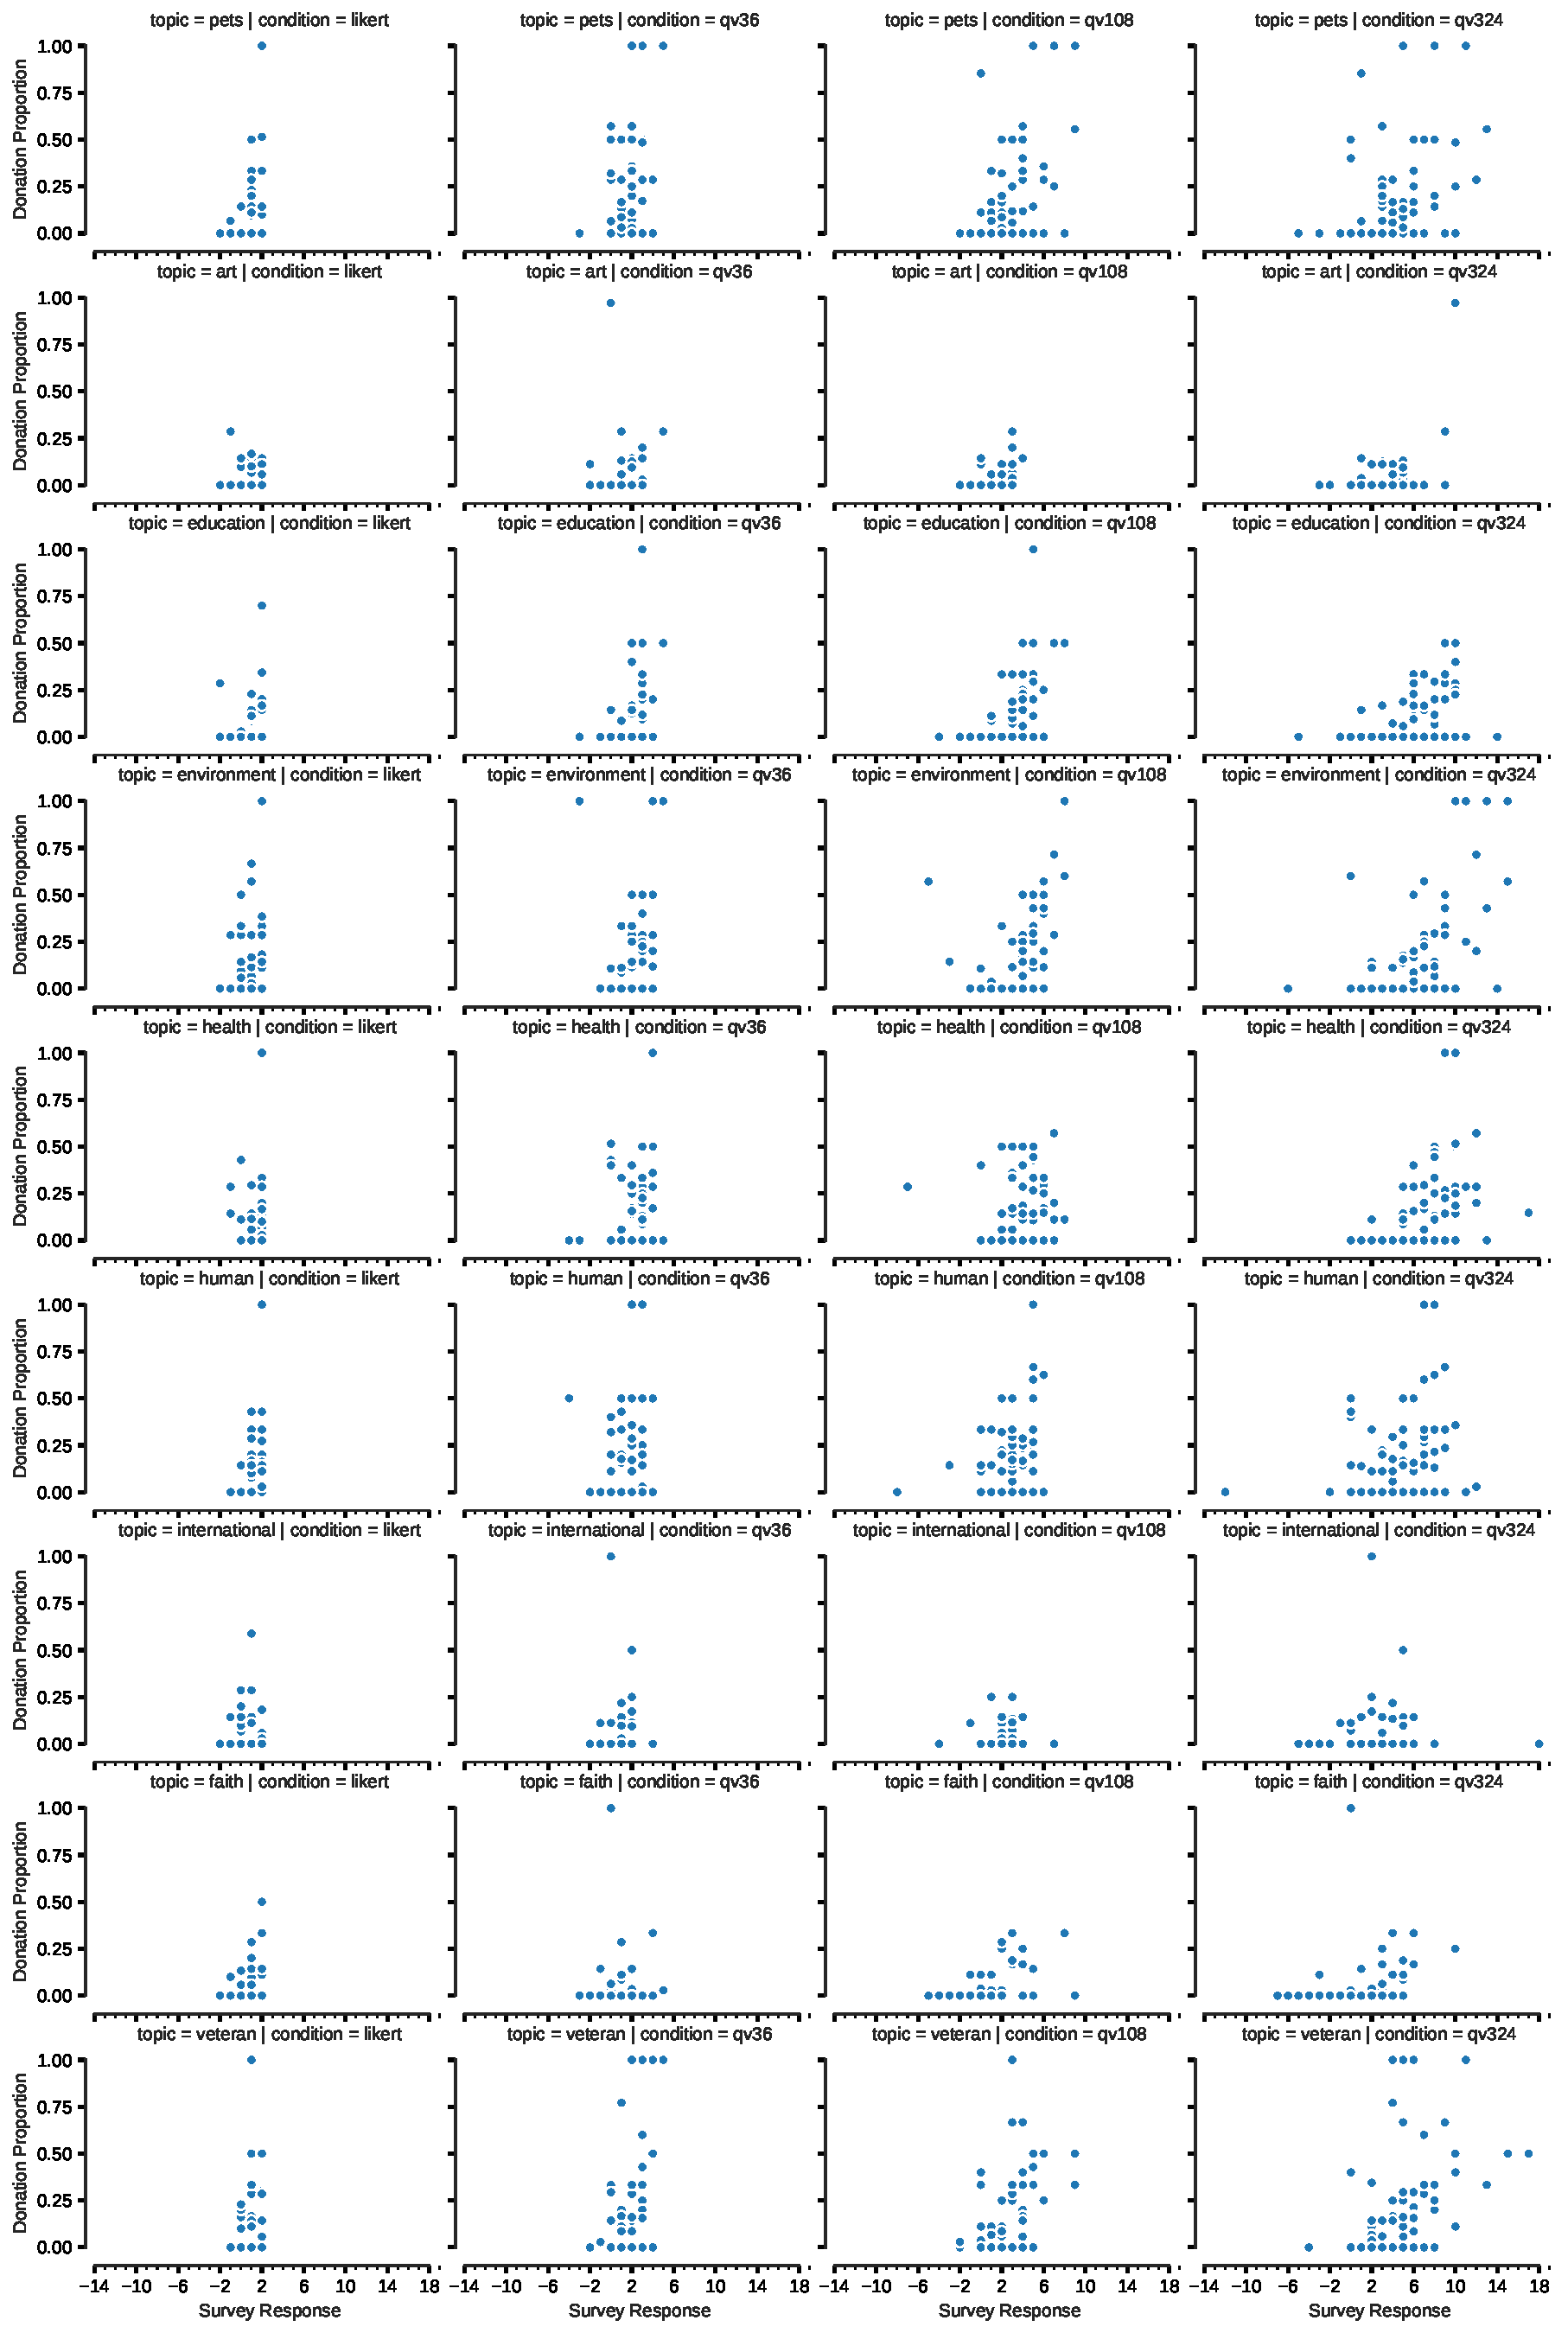
\includegraphics[width=0.85\textwidth, keepaspectratio=true]{content/image/vote_donation_covariates.pdf}
    \caption{
      Scatterplots showing the relationship between participants' normalized survey response and proportional donation amount for nine topics in all four conditions, Likert, QV36, QV108, and QV324. Each row is one topic, and each column is one survey condition. \textbf{The main finding} is: notice that for all subplots, the points showed a positive correlation between survey responses and donation behaviors. We also observed that slopes in the QV plots were more positive than that of Likert in most topics. This observation suggests a stronger correlation between QV survey responses and donation behaviors.
    }
    \Description[Correlation scatterplots between normalized survey response and donation data for experiment one]{
      Scatterplots showing the relationship between participants' survey response and proportional donation amount for each of the nine topics in all four conditions, Likert, QV36, QV108, and QV324.
    }
    \label{fig:topic_covariate_exp1}
\end{figure}



\subsection{Bayesian Analysis Results}
Overall, we concluded from our analysis that survey responses from QV108, QV324 and averaged QV aligned significantly better with the donation results than Likert scale responses with a medium effect size (0.5 - 0.6). 

Recall in \Cref{exp1:The Bayesian Model}, we estimated the posterior distributions of the mean ($\mu_{1-4}$), standard deviation ($\sigma_{1-4}$), and degrees of freedom $\nu$ of the Student-t distributions that characterized the average cosine similarity angle for the four conditions, Likert, QV36, QV108, and QV324. Traceplots of the MCMC chains in~\Cref{fig:traceplot_exp1} show the results of MCMC estimation. The Gelman-Rubin statistic (a measure of MCMC convergence) $\hat{R}$ for all parameters was 1, indicating that the multiple sampling chains converged. 
% To check if the fitted distributions described the data well, please refer to the discussion about posterior predictive check in 

The first graph in the left column of~\Cref{fig:traceplot_exp1} shows that the mean cosine similarity angle of the four conditions varied. In QV108 and QV324 (the overlapping orange and green distributions on the left-most side), the modes of the mean cosine similarity angle (QV108: mode = $44.649 \deg$, QV324: mode = $44.796 \deg$) were smaller than those in the other two conditions, indicating a better alignment between the survey results and donation behavior in QV108 and QV324. The modal value of the average angle in QV36 (mode = $49.029 \deg$, the red distribution in the middle) was slightly higher than that of QV108 and QV324. Likert (the blue line) had the largest model value ($52.857 \deg$) among all four conditions. 
% The posterior distributions of the scale parameter $\sigma$ in all four likelihood functions are similar, with a mode ranging from $13.904$ and $15.724$.

To compare how different the mean cosine similarity angles are statistically between Likert and the three QVs, we constructed the distribution of the absolute difference between the means and the distribution of the corresponding effect size (normalized difference) as shown in \Cref{fig:contrast_exp1}. The first three columns show the absolute difference (top row) and effect size (bottom row) between Likert and each of the three QV conditions. The fourth column compares the Likert condition with the averaged QV condition, by pooling together the responses from three QV conditions. 

\begin{figure}[htpb]
  \centering
  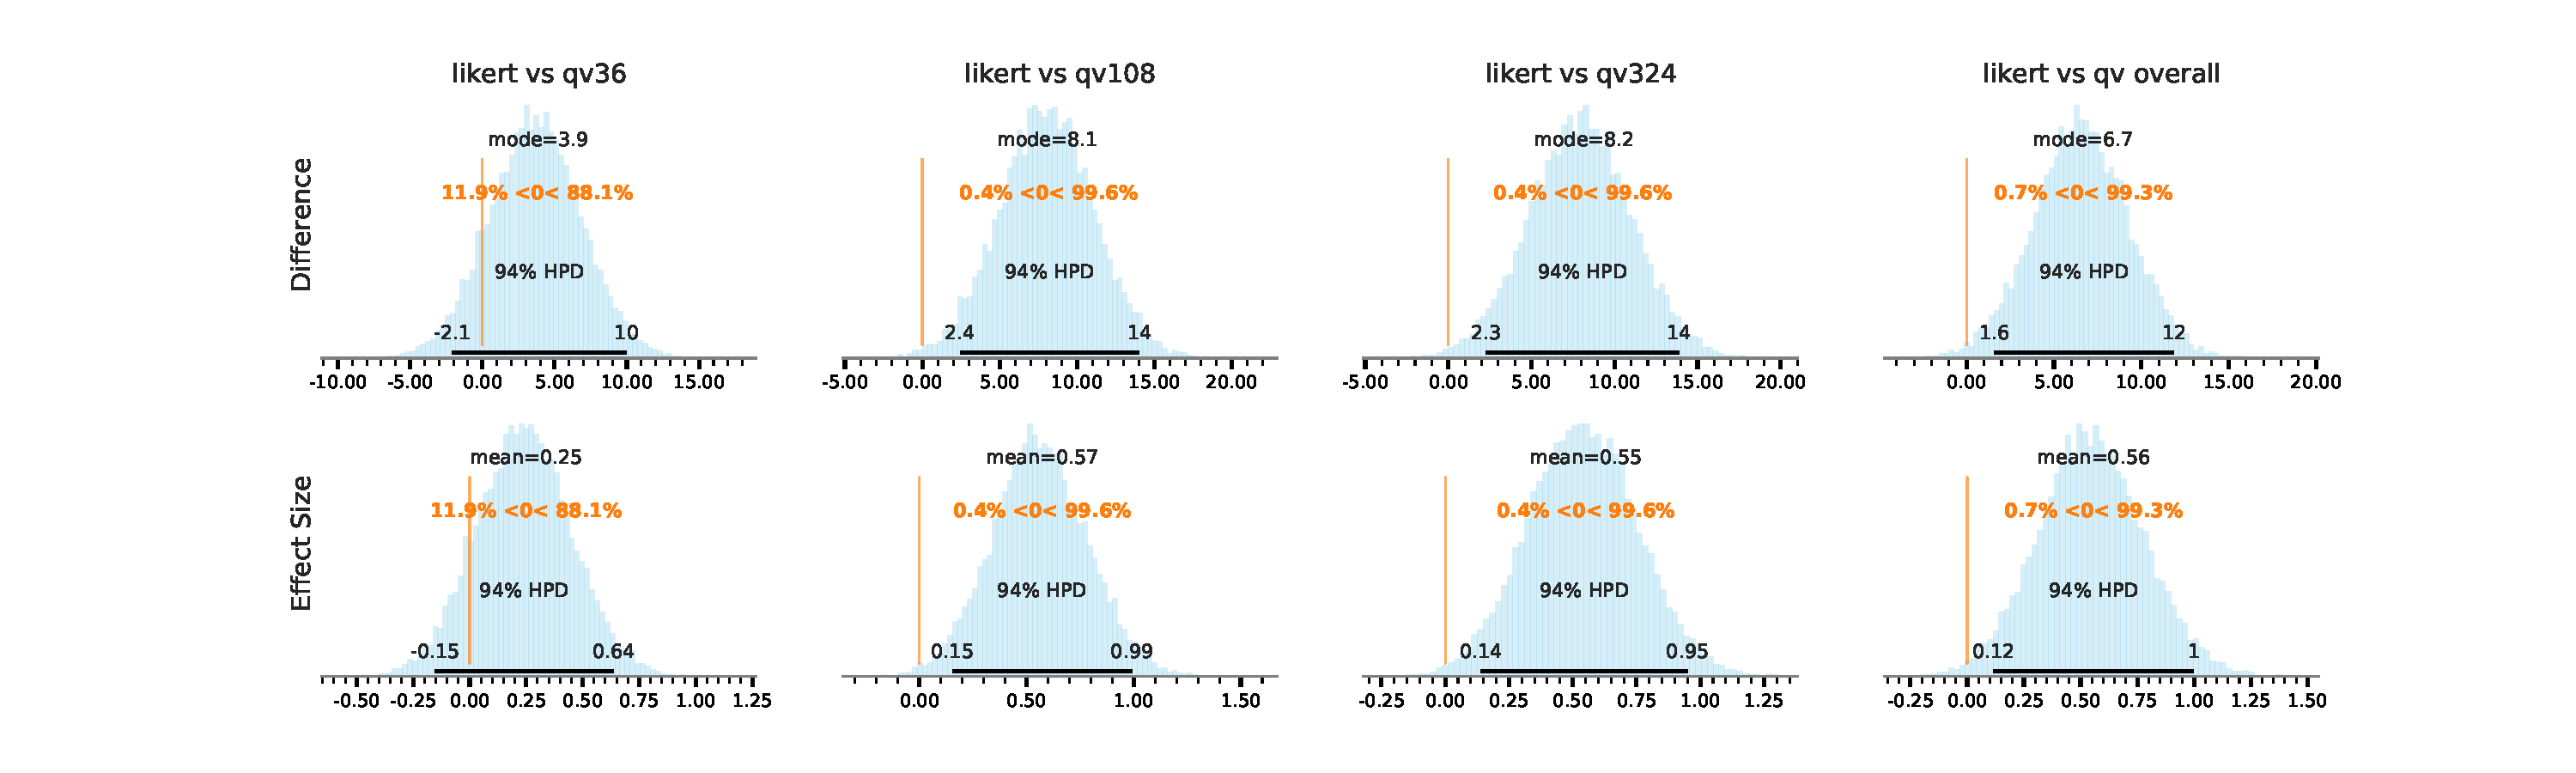
\includegraphics[trim= 2in 0in 2in 0in, clip, width=\textwidth, keepaspectratio=true]{"content/image/Votes_vs_Absolute_Donation_StudentT_differences_and_effects.pdf"}
  \caption{
    The figure shows the contrasts distribution of the mean cosine similarity angles between the four experimental conditions. The four columns show the contrasts between the Likert and QV36, QV108, QV324 and the averaged QV condition respectively. The first row shows the absolute difference while the second row is about the effect size. Since we are highlighting contrasts, each sub-figure shows an orange vertical line located at 0. \textbf{The main finding} is: survey responses from QV108, QV324 and averaged QV aligned significantly better with the donation behaviors than Likert responses with a medium effect size.
  }
  \Description[Contrasts distribution of the mean cosine similarity angles between the four experimental conditions for experiment one]{Contrasts distribution of the mean cosine similarity angles between the four experimental conditions for experiment one}
  \label{fig:contrast_exp1}
\end{figure}

We now examine column $2$ (Likert vs. QV108) in detail, and the rest of the columns follow a similar logic of interpretation. The second column shows the absolute contrast and its effect size of the mean cosine similarity angle between Likert and QV108. The absolute contrast equals to the angles in Likert group subtracted by the angles in QV108. In the top figure of the second column, the mode of the contrast is $8.4$ with the 94\% High Posterior Density (HPD) interval of [$2.6$, $14$]. This means that the cosine similarity angles in the Likert group were most frequently $8.4$ degrees larger than the angles in the QV108 group, i.e., Likert responses were most frequently $8.4$ degrees more misaligned with the donation behaviors than responses from QV108. $94\%$ of the difference in misalignment angles lie between [$2.6 \deg$, $14 \deg$]. Since the HPD lies outside a significant ROPE (Region of Practical Equivalence) of $0 \pm 1 \deg$, there was a significant difference between the alignment levels of the two survey methods. In addition, the bottom figure of the second column shows that the effect size has a modal value of $0.56$, a medium-sized effect\footnote{We use the conventional standard that an effect of 0.2 is considered small, 0.5 is medium, and 0.8 is large.}. The HPD interval of the effect size is [$0.17$, $1$], not overlapping with the ROPE of [$0 \pm 0.1$], which consists of half of the small effect size of 0.2, indicating a statistically significant medium to large effect size.

In the third column, we compare the mean cosine similarity angle of the Likert group
against that of the QV324. The interpretation of this column is very similar to that of the second column above. It has a mode of $8.2$ with a 94\% High Posterior Density (HPD) interval of [$2.5$, $14$] for the contrast. Again, the HPD lies outside the ROPE of $0 \pm 1$ which implies that QV324 responses aligned significantly closer to the donation behaviors than Likert responses. Similarly, the effect size has a mode of $0.56$ with a 94\% HPD interval of [$0.16$, $0.96$], indicating a significant, medium to large-sized effect.

The first column shows a different result. It compares the degree of misalignment of the Likert group against that of QV36. The mode of the contrast is $3.9$, with a 94\% High Posterior Density (HPD) interval of [$-2$, $10$]. While the mode is positive, the HPD interval overlaps with a ROPE of $0 \pm 1$, implying that the observed differences are not significant. The corresponding effect size shows a mode of $0.24$ and a HPD interval of [$-0.13$, $0.66$]. About 11.5\% of the HPD is to the left of zero, also indicating an insignificant effect size. The result suggests that QV survey with only 36 voice credits did not outperform Likert scale survey significantly in terms of alignment with the donation behaviors.

At last, the fourth and final column compares the degree of misalignment with donation behaviors between the Likert group and the averaged QV condition, by pooling three groups of QV together. We see a mode of $6.7$ with an High Posterior Density (HPD) interval of [$1.8$, $12$]. Following the same interpretation logic, the pooled QV condition aligned significantly closer to the donation behaviors than Likert condition. The modal effect size is $0.56$, with an HPD interval of [$0.13$, $0.99$], indicating a significant medium to large effect size.
% The posterior of the pooled QV condition is simply the averages of the values of the posteriors from QV36, QV108 and QV324 for every step in the MCMC, because the MCMC jointly estimates the posteriors of all variables at every step. 


\begin{sidewaysfigure*}
  \centering
  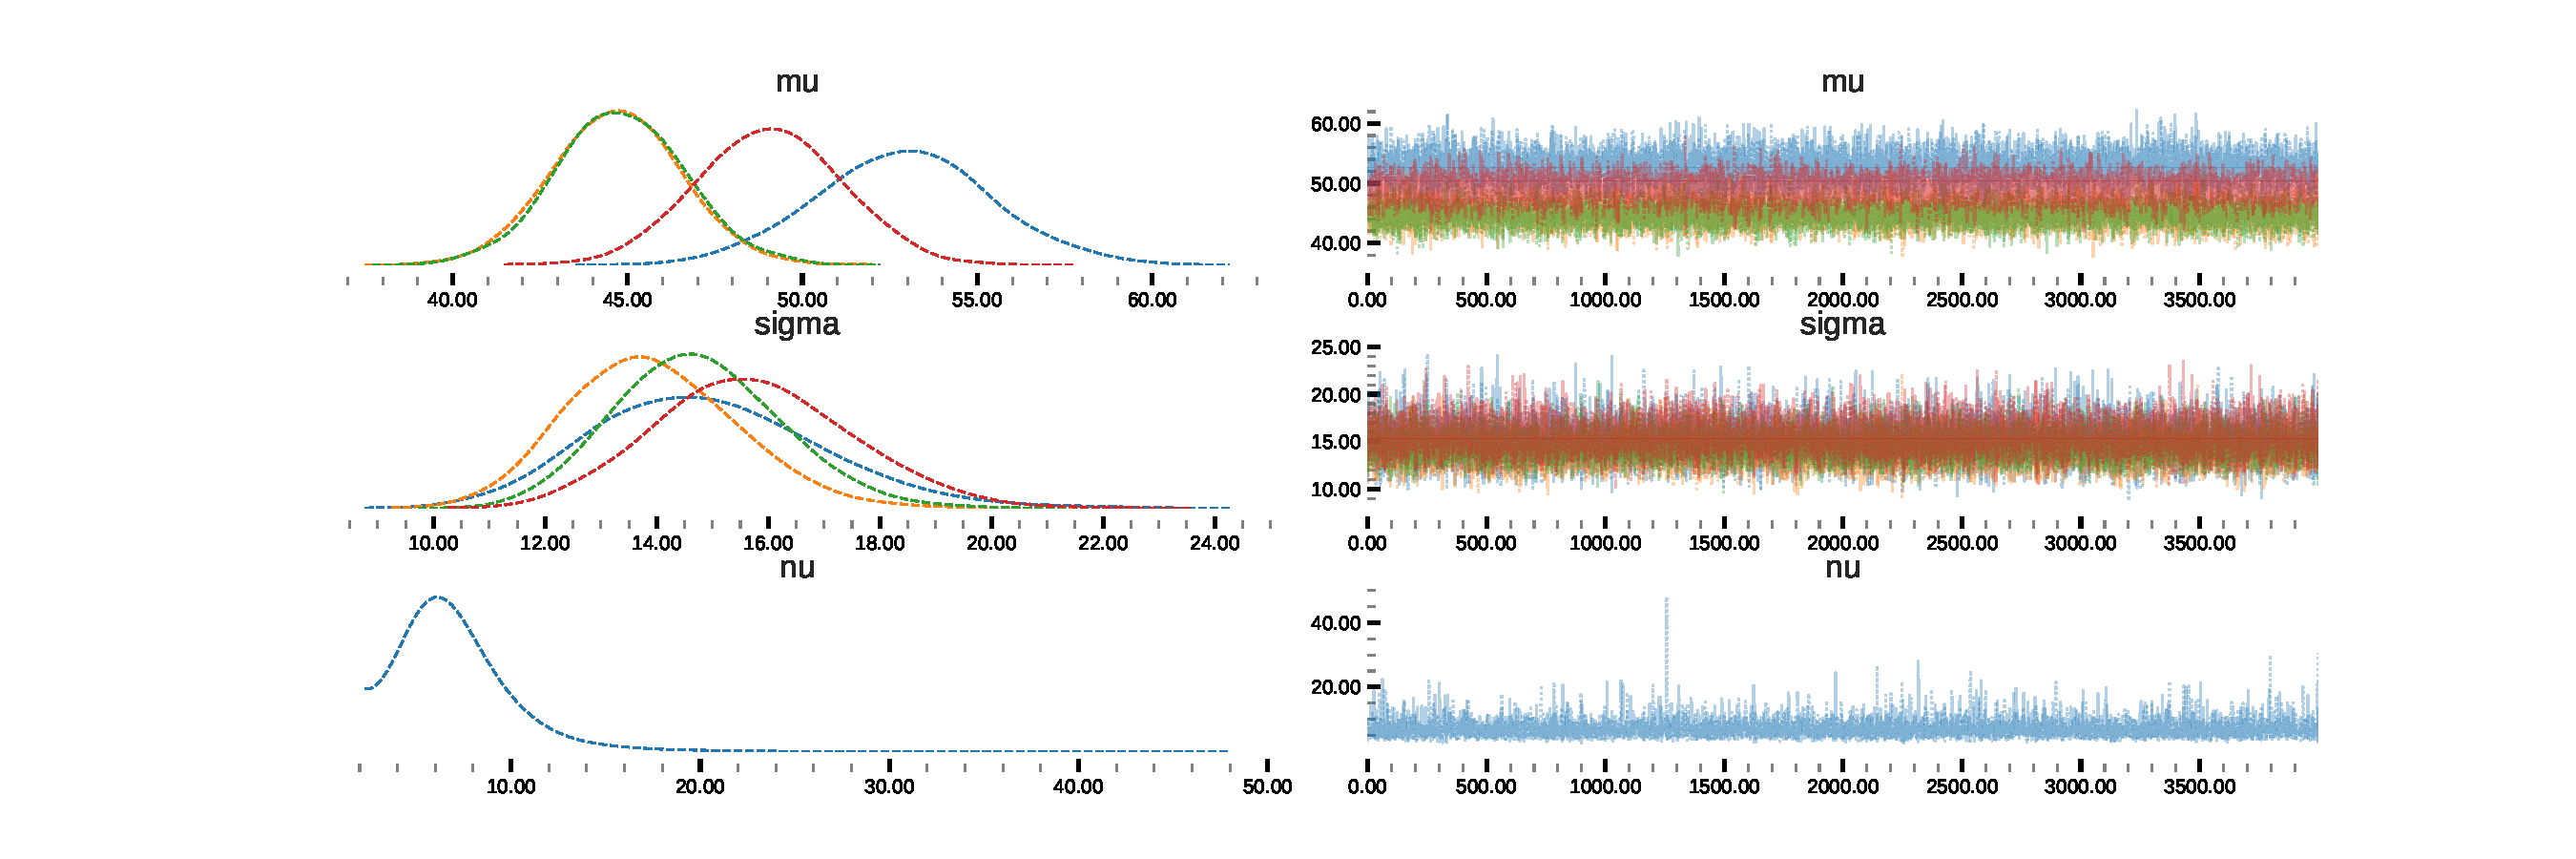
\includegraphics[trim= 2in 0in 2in 0in, clip, width=\textwidth, keepaspectratio=true]{content/image/StudentTIndep_VA_traceplot.pdf}
  \caption{
    Traceplot showing the results of the MCMC estimation in experiment one. The left column is the posterior distributions for $\mu_{1-4}$, $\sigma_{1-4}$, and $\nu$ of the Student-t distribution. The right column shows the corresponding sampling traces. The color mappings are: red (QV36), orange (QV108), green (QV324), blue (Likert). Notice that QV108 and QV324 have similar distributions for $\mu_{1-4}$ and are to the left of QV36 and Likert, meaning a better alignment with donation behaviors. Likert shows the worst alignment: as a reminder, the ideal alignment angle should be $0^o$. Note also, that the modal value for degrees of freedom $\nu \approx 7$, confirming our choice of the Student-t distribution instead of the Normal distribution, which usually requires $\nu \geq 30$. Furthermore, the Gelman-Rubin statistic $\hat{R}$ for all parameters was 1, indicating  convergence of the sampling MCMC chains.
  }
  \Description[Traceplot for the MCMC estimation in experiment one Bayesian model]{Traceplot for the MCMC estimation in experiment one Bayesian model}
  \label{fig:traceplot_exp1}
\end{sidewaysfigure*}



% Similiar claim that QV allows better alignment to ones true preference
% can be supported by Qualitative Analysis Results.
% We ask participants to provide a freeform text response on the reason why they made the choices they made
% when participants filled out the Likert survey or QV survey,
% Of all surveys ($N=394$) across both groups, most participants filled out the surveys ($N=331$) based on what they think are the most important issues to them. %84 percent
% Besides, a small portion of participants ($N=30$) used their instincts when replying to the survey.
% Some participants either think that every aspect is important ($N=7$) or that resources should be equally distributed ($N=7$). 